\chapter{Continuous Models}
Many engineered systems comprise computers, communications networks, and other digital systems to monitor and control physical (electrical, mechanical, thermodynamic, etc.) processes. Models of these systems have some parts modeled as discrete event systems, other parts modeled with continuous (differential or differential-algebraic) equations, and the interaction of these parts is crucial to understanding the system's behavior.

The interaction of continuous and discrete event models is necessarily discrete. For example, a digital thermometer reports temperature in discrete increments, electrical switches are either open or closed, a threshold sensor is either tripped or it is not. Discrete interactions in a combined continuous-discrete event simulation are managed just as before: the models interact by producing output events and reacting to input events.

If, on the other hand, two systems interact continuously, then those interacting parts are modeled with continuous equations. In this case, accurate simulation is greatly facilitated by lumping the two systems into a single assembly. In \adevs\ this assembly is an \classname{Atomic} model that encapsulates the system's continuous dynamics. The essence of this approach to combined simulation in \adevs\ consists therefore of building atomic models that i) approximate the behavior of the continuous systems and ii) generate and consume events at the instants when the continuous system interacts with a discrete event one.

There are three possibly outcomes of this lumping process. One possibility is that we end up with a single assembly. In this case our model is essentially continuous and we are probably better off using a simulation tool for continuous systems. At the other extreme, we find that the continuous parts of our model are very simple, yielding to analytical solutions that are easily transformed into discrete event models. Between these extremes are models with continuous dynamics that are not simple but do not dominate the modeling problem. The continuous system simulation part of \adevs\ is aimed at this type of model.

\section{Differential equation modeling with the \classname{ode\_system} class}
Models described by ordinary differential equations are implemented by sub-classing the \classname{ode\_system} class. This class has two sets of methods: the first is for the model's continuous dynamics and the second is for the model's discrete event dynamics. I'll illustrate both with the simple, if somewhat contrived, example of a cherry bomb\footnote{A cherry bomb is a small red firecracker. They are dangerous and illegal in the United States. Nonetheless, every school seems to have at least one obnoxious kid who likes to put them into the toilets.}. This bomb is dropped from a height of 1 meter and bounces until it explodes or is doused with water. We'll assume that the cherry bomb only bounces up and down and is perfectly elastic. The cherry bomb explodes 2 seconds from the time it is lit unless doused first. Dousing the cherry bomb puts out the fuse\footnote{Cherry bomb fuses are frequently water proofed.}. Dousing is a discrete input event and the cherry bomb produces a discrete output event if it explodes. 

This model has two continuous state variables: the height and the velocity of the cherry bomb. Between events, these variables are governed by the pair of differential equations
\begin{align}
&\dot{v} = -9.8 \label{eqn:v} \\
&\dot{h} = v \label{eqn:h}
\end{align}
where $9.8$ meters per second per second is acceleration due to gravity, $v$ is velocity, and $h$ is height. In this example, it is also useful to know the current time. We keep track of this by adding one more differential equation
\begin{equation}
\dot{t} = 1 \label{eqn:t}
\end{equation}
whose solution is $t_0 + t$ or just $t$ if we set $t_0 = 0$. The ball bounces when it hits the floor, and bouncing causes the ball's velocity to change sign. Specifically
\begin{equation}
h = 0 \ \& \ v < 0 \implies v \leftarrow -v \label{eqn:state_event}
\end{equation}
where $\implies$ is logical implication and $\leftarrow$ indicates an assignment. 

Equations \ref{eqn:v}, \ref{eqn:h}, and \ref{eqn:t} are the state variable derivatives, and these equations are implemented in the \methodname{der\_func} method of the \classname{ode\_system} class. The signature for this method is
\begin{verbatim}
void der_func(const double* q, double* dq)
\end{verbatim}
The q pointer is the array of state variable values: $h$, $v$, and $t$. The dq pointer is the array of state variable derivatives: $\dot{h}$, $\dot{v}$, and $\dot{t}$. When the simulator calls \methodname{der\_func}, it supplies q. In response, the method computes the values of $\dot{h}$, $\dot{q}$, and $\dot{t}$ and stores them in the dq array.

Equation \ref{eqn:state_event} is a state event condition and it is implemented in two parts. The \methodname{state\_event\_func} method implements the `if' part (left hand side) of the condition. The signature of this method is
\begin{verbatim}
void state_event_func(const double *q, double *z)
\end{verbatim}
Again, the supplied q array contains the current state variable values. These are used to evaluate the state event condition and store the result in the z array. The simulator detects state events by looking for changes in the sign of the z array entries. Note that the event condition should be continuous in the state variables on which it depends. In the case of the cherry bomb this is simple to do. We simply use $z=h$ if $v < 0$ and $z=1$ if $v >= 0$.  

The `then' part (right hand side) is implemented with the \methodname{internal\_event} method, which the simulator invokes when the state event condition is true. The signature of this method is
\begin{verbatim}
void internal_event(double *q, const bool *state_event)
\end{verbatim}
where the q array contains the value of the state variables at the event. The entries of the array state\_event are true for each z in the state event condition array that evaluates to zero. This array therefore has one entry for each state event condition, and it has one additional entry to indicate time events, which are described below.

The cherry bomb has one discrete state variable with three possible values: the fuse is lit, the fuse is not lit, and the bomb is exploded. This variable changes in response to two events. The first event is when the bomb explodes. This is a time event that we know will occur 2 seconds from the time that the fuse it lit. The \methodname{time\_event\_func} method is used to schedule the explosion by returning the time remaining until the fuse burns out. The signature of the of this method is
\begin{verbatim}
double time_event_func(const double* q)
\end{verbatim}
As before, the q array has the current value of the state variables. The \methodname{time\_event\_func} is similar to the \methodname{ta} method. It is used to schedule autonomous events based on the current value of the model's state variables. When this time expires, the simulator calls the \methodname{internal\_event} method with the last flag in the state event array set to true.

The second event that can change the state of the fuse is dousing with water. This an external event. External events occur when input arrives at the model. The \methodname{external\_event} method implements the response of the cherry bomb to dousing with water. Its signature is
\begin{verbatim}
void external_event(double *q, double e, const Bag<X> &xb)
\end{verbatim}
The array q contains the values of the continuous state variables, e is the time since the last discrete event, and xb is the bag of input. The douse event is an input and it appears in the input bag xb when and if the event occurs. 

As before, it is possible for an external and internal event to coincide. When this happens, the simulator calls the method \methodname{confluent\_event}. Its signature is
\begin{verbatim}
void confluent_event (double *q, const bool *state_event, const Bag<X> &xb)
\end{verbatim}
and its arguments are as described for the internal and external methods.

The cherry bomb produces an output event when it explodes, and the \methodname{output\_func} method is used for this purpose. Its signature is
\begin{verbatim}
void output_func(const double *q, const bool *state_event, Bag<X> &yb)
\end{verbatim}
The q and state\_event arguments are as described for the \methodname{internal\_event} method, and the bag yb is to be filled with the model's output. As with an \classname{Atomic} model, the \methodname{output\_func} is always invoked immediately prior to the \methodname{internal\_event} and \methodname{confluent\_event} methods.

All that remains in the implementation is the \methodname{gc\_output} for collecting garbage, a constructor, and a method for initializing the continuous state variables. The \methodname{gc\_output} method works identically to that of the \classname{Atomic} class. The constructor for the cherry bomb must call the constructor of its \classname{ode\_system} base class. The signature of this method is
\begin{verbatim}
ode_system (int N_vars, int M_event_funcs)
\end{verbatim}
where N\_vars is the number of entries in the q and dq arrays (i.e., the number of continuous state variables) and M\_event\_funcs is the number of entries in the z and state\_event arrays (plus one for the time event). For the cherry bomb, N\_vars is three and M\_event\_funcs is one.

The constructor for the cherry bomb does not initialize the continuous state variables. Instead, the simulator calls its \methodname{init} method whose signature is
\begin{verbatim}
void init(double* q)
\end{verbatim}
where q is an array that should be filled with the initial values for the continuous variables $h$, $v$, and $t$. The complete implementation of the \classname{CherryBomb} is listed below.
\begin{verbatim}
#include "adevs.h"
#include <iostream>
using namespace std;
using namespace adevs;

// Array indices for the CherryBomb state variables
#define H 0
#define V 1
#define T 2
// Discrete variable enumeration for the CherryBomb
typedef enum { FUSE_LIT, DOUSE, EXPLODE } Phase;

class CherryBomb: public ode_system<string> {
   public:
      CherryBomb():ode_system<string>(
            3, // three state variables including time
            1 // 1 state event condition
            ) {
         phase = FUSE_LIT; // Light the fuse!
      }
      void init(double *q) {
         q[H] = 1.0; // Initial height
         q[V] = 0.0; // Initial velocity
         q[T] = 0.0; // Start time at zero
      }
      void der_func(const double* q, double* dq) {
         dq[V] = -9.8; 
         dq[H] = q[V]; 
         dq[T] = 1.0; 
      }
      void state_event_func(const double* q, double *z) {
         // Test for hitting the ground. 
         if (q[V] < 0.0) z[0] = q[H];
         else z[0] = 1.0;
      }
      double time_event_func(const double* q) {
         if (q[T] < 2.0) return 2.0 - q[T]; // Explode at time 2
         else return DBL_MAX; // Don't do anything after that
      }
      void external_event(double* q, double e, const Bag<string>& xb) {
         phase = DOUSE; // Any input is a douse event
      }
      void internal_event(double* q, const bool* state_event) {
         if (state_event[0]) q[V] = -q[V]; // Bounce!
         if (state_event[1]) phase = EXPLODE;
      }
      void confluent_event(double* q, const bool* state_event,
         const Bag<string>& xb) {
         internal_event(q,state_event);
         external_event(q,0.0,xb);
      }
      void output_func(const double *q, const bool* state_event,
            Bag<string>& yb) {
         if (state_event[1] && phase == FUSE_LIT)
            yb.insert("BOOM!"); // Explode!
      }
      void postStep(const double* q) {
         // Write the current state to std out
         cout << q[T] << " " << q[H] << " " << q[V] << " " << phase << endl;
      }
      // No garbage collection is needed
      void gc_output(Bag<string>&){}
      // Get the current value of the discrete variable
      Phase getPhase() { return phase; } 
   private:
      Phase phase;
};
\end{verbatim}

The \classname{CherryBomb} itself is not derived from \classname{Atomic} and so cannot be simulated directly. Rather, it is given to a \classname{Hybrid} object, which is a kind of \classname{Atomic}, that generators the trajectories for the model. This \classname{Hybrid} object is used just like any other \classname{Atomic} model. Input to this \classname{Hybrid} object triggers an input event for the \classname{ode\_system} that is contains. Likewise, output from the \classname{ode\_system} becomes output from the \classname{Hybrid} object. Most importantly, the hybrid model can be part of any network of discrete event models.

A \classname{Hybrid} object is provided with three things when it is constructed. First is the \classname{ode\_system} itself. Second is an \classname{ode\_solver} that produces the model's continuous trajectories. \adevs\ has two types of \classname{ode\_solvers}: a \classname{corrected\_euler} solver that uses the corrected Euler method and a \classname{rk\_45} solver that uses a fourth/fifth order Runge-Kutta method. Third is an \classname{event\_locator} that finds the location of state events as the simulation progresses. \adevs\ has two these: the \classname{linear\_event\_locator} and \classname{bisection\_event\_locator}. The code below shows how these are used to create and simulate a \classname{Hybrid} object.
\begin{verbatim}
int main() {
   // Create the model
   CherryBomb* bomb = new CherryBomb();
   // Create the ODE solver for this model. Maximum error
   // tolerance at each step is 1E-4 and the maximum
   // size of an integration step is 0.01.
   ode_solver<string>* ode_solve =
      new corrected_euler<string>(bomb,1E-4,0.01);
   // Create the event locator for this model. Maximum
   // error tolerance for the location of an event in
   // the state space is 1E-8.
   event_locator<string>* event_find =
      new linear_event_locator<string>(bomb,1E-8);
   // Create an atomic model that puts all of these
   // together to simulate the continuous system.
   Hybrid<string>* model =
      new Hybrid<string>(bomb,ode_solve,event_find);
   // Create and run a simulator for this model
   Simulator<string>* sim = new Simulator<string>(model);
   while (bomb->getPhase() == FUSE_LIT)
      sim->execNextEvent();
   delete sim; delete bomb;
   return 0;
}
\end{verbatim}

Figure \ref{fig:cherry_bomb_trajectory} shows the cherry bomb's trajectory from $t=0$ to its explosion at $t=2$. This plot was produced using the simulation program listed above. There are two bounce events at $t \approx 0.45$ and $t \approx 1.4$. The cherry bomb explodes abruptly at the start of its third descent.
\begin{figure}[ht]
\centering
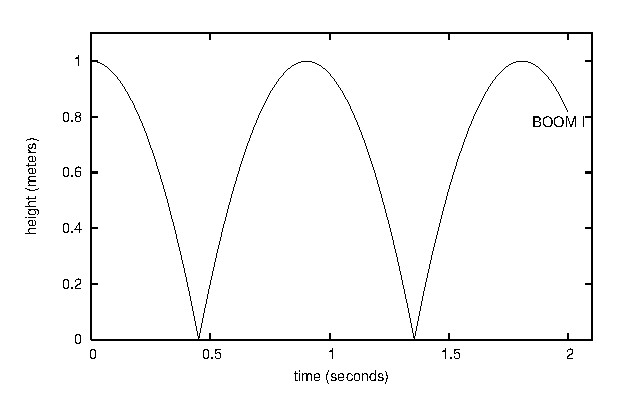
\epsfig{file=cont_models_figs/ball_height.eps}
\caption{A simulation of the cherry bomb model that terminates when the cherry bomb explodes.}
\label{fig:cherry_bomb_trajectory}
\end{figure}

\section{Modeling hybrid systems with the Functional Mockup Interface}
\label{sect:fmi}
The Functional Mockup Interface (FMI) is a standard API for encapsulating piecewise continuous models. The intent of this standard is to allow model developers to exchange their models in a way that is amenable to accurate simulation. The FMI interface specification can be found at \url{http://www.fmi-standard.org}. The practical advantage of this standard for modelers using adevs is that all major Modelica compilers can export their models in this form, and these can be wrapped in an ode\_system object.

You will need three things to use this capability:
\begin{enumerate}
\item The FMI header files, which can be downloaded from the FMI website \url{http://www.fmi-standard.org}.
\item A Modelica compiler or other continuous system modeling tool that will export models in the FMI format.
\item A python interpreter if you want to use the utility script xml2cpp.py (located in the util directory) for generating boiler plate for loading FMI's from the model description files generated by OpenModelica (or any other Modelica compiler that supports FMI).
\end{enumerate}
It is also helpful to have a passing familiarity with the FMI markup language for describing a model. Documentation for this markup language can be found in the FMI standard. This script xml2cpp.py can be used to automated the process described in this section.

The cherry bomb from the previous section will illustrate how the FMI import feature is used. This example can be found in the examples/fmi/Example3 directory. We will create a bomb that begins at its initial height of 1 meter and remains there until it is dropped. Dropping the ball also starts the fuse. The falling and bouncing behavior of the bomb and its explosion after 2 seconds are implemented as a Modelica model. For this example we will omit the dousing. The Modelica code for this model is shown below.
\begin{verbatim}
model CherryBomb
   Real h(start=1); // Height of the bomb
   Real v(start=0); // Velocity of the bomb
   parameter Real g = 9.8; // Gravity
   Real fuseTime(start=2.0); // Fuse duration
   input Boolean dropped(start=false); 
   output Boolean exploded(start=false);
equation
   // Accelerate downward if we have been lit
   der(v) = if (not dropped) then 0 else -g;
   der(h) = v;
   // Burn the fuse
   der(fuseTime) = if (not dropped) then 0 else -1;
   when {h <= 0} then
      reinit(v,-pre(v));
   end when;
   when {fuseTime <= 0} then
      exploded = true;
   end when;
end CherryBomb;
\end{verbatim}

I will use the OpenModelica compiler to demonstrate how this is converted to an FMI compliant object file that can be used with adevs. Assume that the compiler omc is in our path. We begin by creating a Modelica script file called \filename{makefmi.mos} and put into this file the following commands.
\begin{verbatim}
loadFile("CherryBomb.mo");
translateModelFMU(CherryBomb,"2.0");
\end{verbatim}
The first line loads the CherryBomb model that is listed above. The second line generates and FMI object from this model that is compliant with the FMI v2 standard. This FMI object will be packed with several other files in a zipped file called \filename{CherryBomb.fmu}. The OpenModelica compiler will also produce a bunch of other junk that you don't need, and these extra files can be deleted with the following set of command.
\begin{verbatim}
rm -f CherryBomb_*
rm -f CherryBomb.c
\end{verbatim}
To get at the files you need, decompress the zip file with the command
\begin{verbatim}
unzip -o -qq CherryBomb.fmu
\end{verbatim}
This will create directory called \filename{sources}, which you can delete, a file called \filename{modelDescription.xml}, which you will need, and a file \filename{CherryBomb.so}, which you will need. This shared object file will be in the directory called \filename{binaries/linux64}.

The file \filename{modelDescription.xml} contains all of the information you will need to program your simulator to access the variables of the Modelica model. The listing of the description file for the cherry bomb is shown below. The significance of the data in this file will become apparent as we construct the rest of the simulation software that will interact with this model.
\begin{verbatim}
<?xml version="1.0" encoding="UTF-8"?>
<fmiModelDescription
  fmiVersion="2.0"
  modelName="CherryBomb"
  guid="{8c4e810f-3df3-4a00-8276-176fa3c9f9e0}"
  description=""
  generationTool="OpenModelica Compiler 1.9.2+dev (r24043)"
  generationDateAndTime="2015-02-08T18:41:22Z"
  variableNamingConvention="structured"
  numberOfEventIndicators="3">
  <ModelExchange
    modelIdentifier="CherryBomb">
  </ModelExchange>
  <TypeDefinitions>
  </TypeDefinitions>
  <LogCategories>
    <Category name="logEvents" />
    <Category name="logSingularLinearSystems" />
    <Category name="logNonlinearSystems" />
    <Category name="logDynamicStateSelection" />
    <Category name="logStatusWarning" />
    <Category name="logStatusDiscard" />
    <Category name="logStatusError" />
    <Category name="logStatusFatal" />
    <Category name="logStatusPending" />
    <Category name="logAll" />
    <Category name="logFmi2Call" />
  </LogCategories>
  <DefaultExperiment startTime="0.0" stopTime="1.0" tolerance="1e-06"/>
  <ModelVariables>
  <!-- Index of variable = "1" -->
  <ScalarVariable
    name="fuseTime"
    valueReference="0"
    variability="continuous"
    causality="local"
    initial="approx">
    <Real start="2.0"/>
  </ScalarVariable>
  <!-- Index of variable = "2" -->
  <ScalarVariable
    name="h"
    valueReference="1"
    variability="continuous"
    causality="local"
    initial="approx">
    <Real start="1.0"/>
  </ScalarVariable>
  <!-- Index of variable = "3" -->
  <ScalarVariable
    name="v"
    valueReference="2"
    variability="continuous"
    causality="local"
    initial="approx">
    <Real start="0.0"/>
  </ScalarVariable>
  <!-- Index of variable = "4" -->
  <ScalarVariable
    name="der(fuseTime)"
    valueReference="3"
    variability="continuous"
    causality="local"
    initial="calculated">
    <Real derivative="1"/>
  </ScalarVariable>
  <!-- Index of variable = "5" -->
  <ScalarVariable
    name="der(h)"
    valueReference="4"
    variability="continuous"
    causality="local"
    initial="calculated">
    <Real derivative="2"/>
  </ScalarVariable>
  <!-- Index of variable = "6" -->
  <ScalarVariable
    name="der(v)"
    valueReference="5"
    variability="continuous"
    causality="local"
    initial="calculated">
    <Real derivative="3"/>
  </ScalarVariable>
  <!-- Index of variable = "7" -->
  <ScalarVariable
    name="g"
    valueReference="6"
    variability="fixed"
    causality="parameter"
    initial="exact">
    <Real start="9.800000000000001"/>
  </ScalarVariable>
  <!-- Index of variable = "8" -->
  <ScalarVariable
    name="_D_whenCondition1"
    valueReference="0"
    variability="discrete"
    causality="local"
    initial="calculated">
    <Boolean/>
  </ScalarVariable>
  <!-- Index of variable = "9" -->
  <ScalarVariable
    name="_D_whenCondition2"
    valueReference="1"
    variability="discrete"
    causality="local"
    initial="calculated">
    <Boolean/>
  </ScalarVariable>
  <!-- Index of variable = "10" -->
  <ScalarVariable
    name="dropped"
    valueReference="2"
    variability="discrete"
    causality="input"
    initial="approx">
    <Boolean start="false"/>
  </ScalarVariable>
  <!-- Index of variable = "11" -->
  <ScalarVariable
    name="exploded"
    valueReference="3"
    variability="discrete"
    causality="output"
    initial="approx">
    <Boolean start="false"/>
  </ScalarVariable>
  </ModelVariables>
  <ModelStructure>
    <Outputs>
      <Unknown index="11" dependencies="1" dependenciesKind="dependent" />
    </Outputs>
    <Derivatives>
      <Unknown index="4" dependencies="10" dependenciesKind="dependent" />
      <Unknown index="5" dependencies="3" dependenciesKind="dependent" />
      <Unknown index="6" dependencies="10" dependenciesKind="dependent" />
    </Derivatives>
    <InitialUnknowns>
    </InitialUnknowns>
  </ModelStructure>
</fmiModelDescription>
\end{verbatim}

We will embed this model in a simple simulation program that has two components: the bomb and a separate model that lights the fuse and reports the explosion. The mischievous miscreant that lights the fuse and chuckles when it goes off is described with an atomic model just like those that we've seen before. Its source code is listed below.
\begin{verbatim}
/**
 * A miscreant drops the ball and reports the explosion.
 */
class Miscreant:
   public adevs::Atomic<std::string>
{
   public:
      Miscreant():
         adevs::Atomic<std::string>(),
         start(true),
         tstart(1.0)
      {
      }
      double ta() { return ((start) ? tstart : adevs_inf<double>()); }
      void delta_int() { start = false; }
      void delta_ext(double e, const Bag<std::string>& xb)
      {
         cout << (tstart+e) << " " << (*(xb.begin())) << endl;
      }
      void delta_conf(const Bag<std::string>&){}
      void output_func(Bag<std::string>& yb)
      {
         if (start) yb.insert("light");
      }
      void gc_output(Bag<std::string>&){}
   private:
      bool start;
      const double tstart;
};
\end{verbatim}

Our next goal will be to create code for the CherryBomb model that appears in the main function of the simulation program. As you can see from the code below, this model is used just like any other model that is derived from the ode\_system class, and can be coupled to atomic and other models just like any other component in a simulation program.
\begin{verbatim}
int main()
{
   // Create our model of the bomb
   CherryBomb* bomb = new CherryBomb();
   // Wrap a set of solvers around it
   Hybrid<std::string>* hybrid_model =
      new Hybrid<std::string>
      (
         bomb, // Model to simulate
         new corrected_euler<std::string>(bomb,1E-5,0.01), // ODE solver
         new discontinuous_event_locator<std::string>(bomb,1E-5) // Event locator
         // You must use this event locator for OpenModelica because it does
         // not generate continuous zero crossing functions
      );
   // Couple the miscreant and the bomb
   SimpleDigraph<std::string>* model = new SimpleDigraph<std::string>();
   Miscreant* miscreant = new Miscreant();
   model->add(miscreant);
   model->add(hybrid_model);
   model->couple(miscreant,hybrid_model);
   model->couple(hybrid_model,miscreant);
   // Create the simulator
   Simulator<std::string>* sim =
      new Simulator<std::string>(model);
   // Run the simulation for ten seconds
   while (sim->nextEventTime() <= 4.0)
   {
      cout << sim->nextEventTime() << " ";
      sim->execNextEvent();
      cout << bomb->get_height() << " " << bomb->get_fuse() << endl;
   }
   // Cleanup
   delete sim;
   delete hybrid_model;
   // Done!
   return 0;
}
\end{verbatim}

The CherryBomb class is constructed as a subclass of the adevs FMI class. The FMI class contains all of the instructions needed to load, initialize, update, and access the variables of an FMI v2 object. The construction of the FMI class requires four arguments:
\begin{enumerate}
\item The model name that appears in the \filename{modelDescription.xml} within the tag "modelName".
\item The GUID string for the FMI object that appears within the tag "guid" just beneath "modelName" in \filename{modelDescription.xml}.
\item The number of continuous state variables in the Modelica model, which is determined by counting the number of variable descriptions containing the tagged "Real derivative". There are three of these for the CherryBomb model.
\item The number of state event conditions in the model, which is contained in the tag "numberOfEventIndicators". 
\item The name of the shared object file that contains the equations, etc. for the compiled Modelica model.
\end{enumerate}
The CherryBomb class inherits the functions of the ode\_system class described in the previous section, and the default implementation of these methods by the FMI class is sufficient to simulate the parts of the model's behavior that are described in the Modelica file. If these methods are overridden, then it is necessary to first invoke the method of the base class before performing any other action. If any of the Modelica variables are modified by the overridden method, then it is also necessary to invoke the method of the base class after the modifications have been made. Variables that are part of the Modelica model can be read and written using methods inherited from the FMI class. These methods have the forms \methodname{set\_int(int index, int val)}, \methodname{get\_int(int index): int}, \methodname{set\_double(int index, double val)}, \methodname{get\_double(int index): double}, \methodname{set\_bool(int index, bool val)}, and \methodname{get\_bool(int index): bool}. The index variable for each method should be valueReference number that appears in the file \filename{modelDescription.xml}. Each of these elements is illustrated in the implementation of the CherryBomb class below.

\begin{verbatim}
class CherryBomb:
   // Derive model from the adevs FMI class
   public FMI<std::string>
{
   public:
      // Constructor loads the FMI
      CherryBomb():
         // Call FMI constructor
         FMI<std::string>
         (
            "CherryBomb", // model name from modelDescription.xml
            "{8c4e810f-3df3-4a00-8276-176fa3c9f9e0}", // GUID from modelDescription.xml
            3, // Number of derivative variables
            3, // numberOfEventIndicators from modelDescription.xml
            "binaries/linux64/CherryBomb.so" // Location of the shared object file produced by omc
         )
      {
      }
      // Internal transition function
      void internal_event(double* q, const bool* state_event)
      {
         // Call the method of the base class
         FMI<std::string>::internal_event(q,state_event);
      }
      // External transition function
      void external_event(double* q, double e, const Bag<std::string>& xb)
      {
         // Call the method of the base class
         FMI<std::string>::external_event(q,e,xb);
         // Drop the ball
         set_dropped();
         // Call the base class method again to 
         // recalculate variables that depend on
         // the dropped variable
         FMI<std::string>::external_event(q,e,xb);
      }
      // Time remaining to the next sample
      double time_event_func(const double* q)
      {
         // Return the value of the base class
         return FMI<std::string>::time_event_func(q);
      }
      // Print state at each output event
      void output_func(const double* q, const bool* state_event, Bag<std::string>& yb)
      {
         // Output on the state event that is the explosion.
         // The state event number is in modelDescription.xml
         // as a whenCondition variable.
         if (state_event[1])
            yb.insert("boom!");
      }
      // The exploded variable in the Modelica model is its 
      // third boolean variable. This information is in the
      // modelDescription.xml file generated by the Modelica
      // compiler.
      bool get_exploded() { return get_bool(3); }
      // See modelDescription.xml
      double get_height() { return get_real(1); }
      // See modelDescription.xml
      void set_dropped() { set_bool(2,true); }
      // See modelDescription.xml
      bool get_dropped() { return get_bool(2); }
      // See modelDescription.xml
      double get_fuse() { return get_real(0); }
};
\end{verbatim}

